\section{BACKGROUND}

ISAR imaging requires translational motion compensation and rotational motion compensation. Translational motion compensation is typically regarded as trivial and does not add anything outside of undesirable blurring. Assuming the translational motion compensation has been appropriately applied, Figure \ref{fig:geo} depicts the geometry of the target during ISAR imaging where the target is rotating between pulses.

\subsection{Target Geometry}

The crossrange resolution of ISAR images is dictated by the rotation of the target. Assuming translational motion compensation has been applied, this reduces the ISAR model to a tabletop, where the target rotates at a fixed position away from the radar. Additionally, for the purposes of specifically evaluating the effects of non-uniform sampling and slow-time undersampling, the rotation motion parameters are assumed to be known. Figure \ref{fig:geo} depicts the ISAR imaging geometry.

\begin{figure}[h]
  \centering
  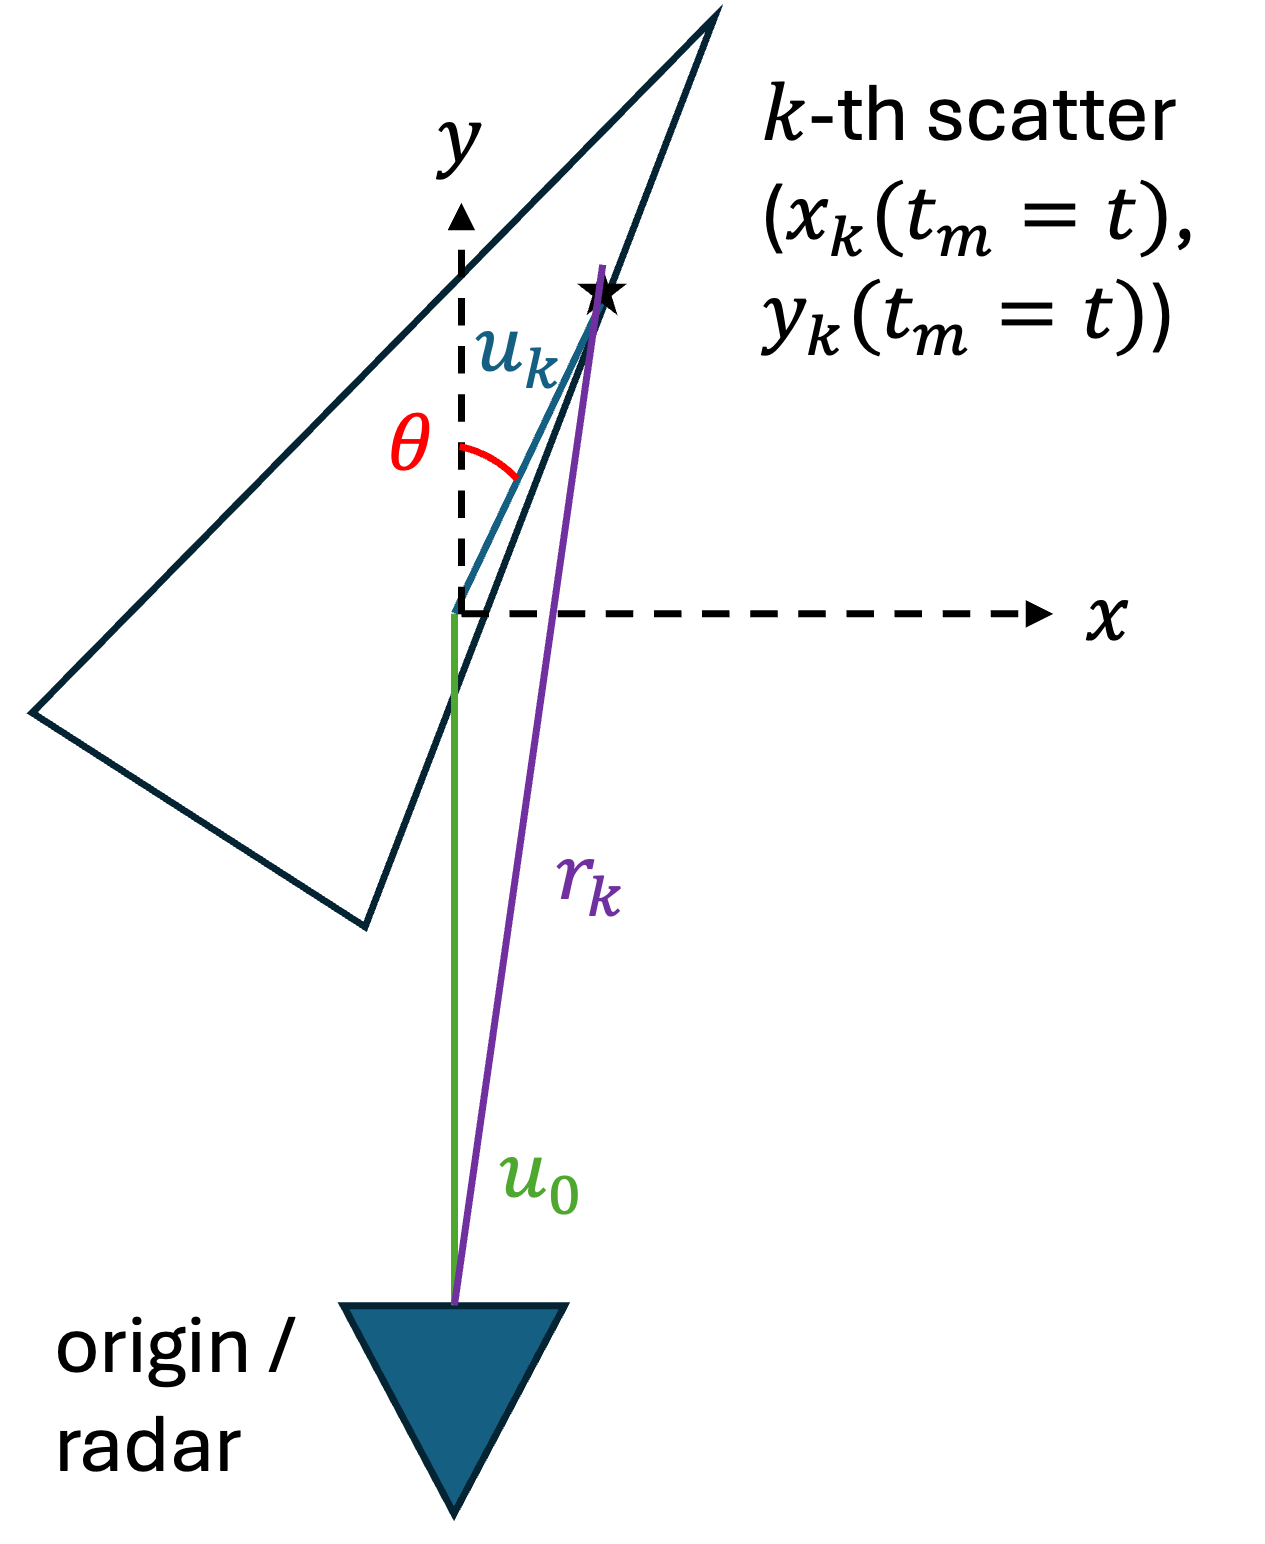
\includegraphics[width=0.3\linewidth]{figures/isar_geo2.png}
  \caption{ISAR target geometry as a function of slow-time}
  \label{fig:geo}
\end{figure}

\noindent The relative position of a scattering point as a function of slow-time ($t_{m}$) can be defined as \cite{Xu2022}:

\begin{equation}
    \begin{bmatrix}
        x_{k}(t_m)\\
        y_k (t_m)
    \end{bmatrix}
    =
    \begin{bmatrix}
        \cos(\theta(t_m)) & -\sin(\theta(t_{m})) \\
        \sin(\theta(t_m)) & \cos(\theta(t_m))
    \end{bmatrix}
    \begin{bmatrix}
        x_{k}\\
        y_k
    \end{bmatrix}
\end{equation}


\noindent where $\theta(t_{m})$ or $\theta_m$ is the angle of the target scatterer relative to the $y$-axis, and $[x_{k}, y_{k}]^{T}$ is the initial position of the $k$-th scatterer relative to the center of the rotation of the target. The range from the origin located at the radar to a scattering point is \cite{Xu2022}:
\begin{equation}
    \begin{aligned}
        r_{k}(t_m) &= \sqrt{x_{k}^2(t_m) + (y_k(t_{m}) + u_{0})^2}\\
        &\approx u_{0} + y_{k}(t_m) \quad \mathrm{as} \quad (y_k(t_{m}) + u_{0})^2 >> x_{k}^2(t_m)\\
        &= u_{0} + x_{k} \sin(\theta(t_{m})) + y_{k}\cos(\theta(t_{m}))\\
        &= u_{0} + u_{k} \\ &\mathrm{where} \quad u_{k} = x_{k} \sin(\theta(t_{m})) + y_{k}\cos(\theta(t_{m}))
    \end{aligned} 
    \label{eq:r}
\end{equation}

\noindent The angle $\theta_m$ can be approximated using a Taylor series:

\begin{equation}
    \begin{aligned}
        \sin(\theta) &= \theta - \frac{\theta^3}{3!} + \frac{\theta^{5}}{5!} + \dots \\
        \cos(\theta) &= 1 - \frac{\theta^2}{2!} + \frac{\theta^{4}}{4!} + \dots
    \end{aligned}
\end{equation}

\noindent For most ISAR applications, the target's rotation is relatively small across the coherent integration time, enabling the usage of the small angle approximation: $\sin(\theta(t_{m})) \approx\theta(t_{m})$ and $\cos(\theta(t_m)) \approx 1$. The range from the radar to a target scatterer can be approximated as:

\begin{equation}
  \begin{aligned}
    r_{k}(t_{m}) &\approx u_{0} + y_{k} + x_{k}\theta_{m} \\ \theta(t_{m}) &= \theta(0) + \omega t_{m} + \frac{\dot{\omega}}{2}t_{m}^{2} + \dots
  \end{aligned}
  \label{eq:r_final}
\end{equation}

\subsection{Signal Model and Sensing Matrix} \label{sec:signal} 

% target geometry
 The signal can be represented as a range-compressed echo:

\begin{equation}
    s(\hat{t},t_{m}) = C \cdot \text{sinc}(B(\hat{t} - \tau(t_{m})))\cdot \exp(-j2 \pi f_{c} \tau(t_{m}))
\end{equation}

\noindent where $C$ is the amplitude, $B$ is the bandwidth, $\hat{t}$ is the fast-time, $t_{m}$ is the slow-time, $\tau$ is the propagation delay and $f_{c}$ is the center frequency. The propagation delay for a monostatic radar configuration is the amount of time required to propagate to the target and return:

\begin{equation}
    \tau_{m} = \frac{2r(t_{m})}{c}
\end{equation}

\noindent where $r(t_{m})$ is the range or distance from the radar to a target scattering point as defined by equation \ref{eq:r}. The return echo can be represented as a summation of the returns from each scatterer:

\begin{equation}
    s(\hat{t},t_{m}) = C \sum_{k} \sigma_{k} \cdot \delta(\hat{t} - \tau_{k}(t_{m})) \cdot \exp(-j2 \pi f_{c} \tau_{k}(t_{m}))
\end{equation}

\noindent where $k$ is the index of each scatterer located at $\delta(\hat{t} - \tau_{k}(t_{m}))$, $K$ is the total number of scatterers or sparsity, and $\sigma_{k}$ is the complex reflectivity of the $k$-th scatterer. Typical formulations will assume separability in the range and crossrange to simplify the sensing matrix's formulation; however, this approach neglects the cross-terms inherent to range-cell migration. To preserve this effect while still defining a linear system suitable for reconstruction using compressed sensing, apply the Fourier transform in the fast-time:

\begin{equation}
    S(\hat{f},t_{m}) = C \sum_{k} \sigma_{k} \cdot \exp(-j2 \pi (f_{c} + \hat{f}) \tau_{k}(t_{m}))
    \label{eq:S}
\end{equation}

\noindent where $\hat{f}$ is the temporal-frequency or the range-frequency. Equation \ref{eq:S} enables a formulation of a sensing matrix where each entry can be defined as:

\begin{equation}
    A[{m + \ell M}, k] = C \sigma_{k} \cdot \exp(-j2 \pi (f_{c} + \hat{f}_{\ell}) \tau_{k}(t_{m}))
\end{equation}

\noindent The resulting linear system is defined as: $y = Ax + n$, where $y \in \mathbb{C}^{ML}$ is the measurement, $A \in \mathbb{C}^{ML \times K}$ is the sensing matrix, and $x \in \mathbb{C}^{K}$ is the vectorized latent image. The dimensionality of the system is determined by the number of range-frequency samples $L$, the number of scatterers $K$ and the number of received pulses $M$ which is less than the number of total pulses $N$ such that $M << N$. Figure \ref{fig:sensing_matrix} depicts the dimensionality of the proposed sensing matrix. 

\begin{figure}[h]
  \centering
  
\includegraphics[width=0.4\linewidth]{figures/linear_sys1.png}
  \caption{Linear system formulation and dimensionality}
  \label{fig:sensing_matrix}
\end{figure}

This system is underdetermined and has infinitely many solutions, each existing in the ($N-M$)-dimensional null space of the sensing matrix. However, to treat this as a compressed sensing problem, if the latent image can be assumed $K$-sparse or containing $K$ non-zero values, the problem becomes $K$-dimensional where $M \geq K$. Additionally, if the sensing matrix is roughly orthogonal and incoherent, associated with the Restricted Isometric Property (RIP), the solution can be unique \cite{Majumdar_2018}. The compressed sensing problem can then be formulated as:

\begin{equation}
    \min_{x} ||x||_{0} \quad \text{subject to} \quad y = Ax
    \label{eq:l0}
\end{equation}

\subsection{OMP}
\label{sec:omp}
There are many different compressed sensing techniques, and Greedy algorithms like Orthogonal Matching Pursuit (OMP) are effective for non-linear recovery \cite{Bostock_2017}. For a Hermitian sensing matrix ($A$) where $A^{-1} = A^{H}$, OMP iterates through a defined sparsity ($K$) and finds the indices ($\Lambda$) that maximize the projection of the residual, initialized as the measurement, onto the basis vectors formed by $A$. The maximization of the residual selects the coefficients projected on the basis vectors formed by $A$, and the step $r = y - A \hat{X}$ prevents the re-selection of the same indices. The latent image estimation $\hat{X}$ is the least-squares approximation formed from the selected basis vectors of $A$. Algorithm \ref{algo:OMP} formally describes the OMP algorithm \cite{Majumdar_2018}.

\begin{algorithm}[H]
\caption{Orthogonal Matching Pursuit}\label{algo:OMP}
\begin{algorithmic}[1]
\Procedure{OMP}{$H,N$}
\State $\Lambda\gets []$
\State $r \gets y$
\State $\hat{X} \gets 0$
\For{$i \leq K$}
\State $c\gets A^{H}r$
\State $\Lambda = \arg\max_{i} \big| c_i \big|$
\State $\Lambda \gets \begin{bmatrix} \Lambda \\ l \end{bmatrix}$
\State $\hat{X} \gets (A(\Lambda)^{H}A(\Lambda))^{-1}A(\Lambda)^{H}y$
\State $r \gets y - A\hat{X}$
\State $i \gets i + 1$
\EndFor
\State \textbf{return} $\hat{X}$
\EndProcedure
\end{algorithmic}
\end{algorithm}